\section{导数}

\begin{problem}{函数在特定点的可导性判定}{Differentiability-At-A-Point}
    讨论下列函数在点 $x = 0$ 处是否可导：
    \begin{enumerate}
        \item $f(x) = |\sin x|$；
        \item $f(x) = \begin{cases} x + 1, & x \geqslant 0, \\ 1, & x < 0; \end{cases}$
        \item $f(x) = \begin{cases} x^2 \sin \frac{1}{x}, & x \neq 0, \\ 1, & x = 0; \end{cases}$
        \item $f(x) = \begin{cases} \ln(1 + x), & x \geqslant 0, \\ x + 1, & x < 0; \end{cases}$
        \item $f(x) = |x|\e^x$；
        \item $f(x) = |x^3|$．
    \end{enumerate}
\end{problem}

\begin{solution}
    \ansitem{1} 不可导．

    计算在 $x = 0$ 处的单侧导数：
    \begin{equation}
        f'_+(0) = \lim_{x\to 0^+} \frac{|\sin x| - 0}{x} = \lim_{x\to 0^+} \frac{\sin x}{x} = 1,
    \end{equation}
    \begin{equation}
        f'_-(0) = \lim_{x\to 0^-} \frac{|\sin x| - 0}{x} = \lim_{x\to 0^-} \frac{-\sin x}{x} = -1.
    \end{equation}
    因 $f'_+(0) \neq f'_-(0)$，故函数在 $x = 0$ 处不可导．
    \begin{equation}
        \boxed{\text{在 } x = 0 \text{ 处不可导．}}
    \end{equation}

    \ansitem{2} 不可导．

    此时 $f(0) = 1$，计算单侧导数：
    \begin{equation}
        f'_+(0) = \lim_{x\to 0^+} \frac{(x + 1) - 1}{x} = 1,
    \end{equation}
    \begin{equation}
        f'_-(0) = \lim_{x\to 0^-} \frac{1 - 1}{x} = 0.
    \end{equation}
    因 $f'_+(0) \neq f'_-(0)$，故函数在 $x = 0$ 处不可导．
    \begin{equation}
        \boxed{\text{在 } x = 0 \text{ 处不可导．}}
    \end{equation}

    \ansitem{3} 不可导．

    因为
    \begin{equation}
        \lim_{x\to 0} f(x) = \lim_{x\to 0} x^2 \sin \frac{1}{x} = 0 \neq f(0) = 1,
    \end{equation}
    函数在 $x = 0$ 处不连续，故不可导．
    \begin{equation}
        \boxed{\text{在 } x = 0 \text{ 处不可导．}}
    \end{equation}

    \ansitem{4} 不可导．

    此时 $f(0) = \ln 1 = 0$，但
    \begin{equation}
        \lim_{x\to 0^-} f(x) = \lim_{x\to 0^-} (x + 1) = 1 \neq f(0),
    \end{equation}
    函数在 $x = 0$ 处不连续，故不可导．
    \begin{equation}
        \boxed{\text{在 } x = 0 \text{ 处不可导．}}
    \end{equation}

    \ansitem{5} 不可导．

    计算单侧导数：
    \begin{equation}
        f'_+(0) = \lim_{x\to 0^+} \frac{x\e^x - 0}{x} = \lim_{x\to 0^+} \e^x = 1,
    \end{equation}
    \begin{equation}
        f'_-(0) = \lim_{x\to 0^-} \frac{-x\e^x - 0}{x} = \lim_{x\to 0^-} (-\e^x) = -1.
    \end{equation}
    因 $f'_+(0) \neq f'_-(0)$，故函数在 $x = 0$ 处不可导．
    \begin{equation}
        \boxed{\text{在 } x = 0 \text{ 处不可导．}}
    \end{equation}

    \ansitem{6} 可导．

    计算导数极限：
    \begin{equation}
        f'(0) = \lim_{x\to 0} \frac{|x^3| - 0}{x} = \lim_{x\to 0} \left( x |x| \right) = 0.
    \end{equation}
    故函数在 $x = 0$ 处可导，且导数值为 $0$．
    \begin{equation}
        \boxed{\text{在 } x = 0 \text{ 处可导，且 } f'(0) = 0.}
    \end{equation}
\end{solution}

\begin{problem}{分段函数处处可导的参数确定}{Piecewise-Function-Differentiability-Parameters}
    求 $a, b$ 的值，使下列函数处处可导：
    \begin{enumerate}
        \item $f(x) = \begin{cases} x^2, & x \leqslant 1, \\ ax + b, & x > 1; \end{cases}$
        \item $f(x) = \begin{cases} \ln(1 + x), & x < 0, \\ ax + b, & x \geqslant 0. \end{cases}$
    \end{enumerate}
\end{problem}

\begin{solution}
    \ansitem{1}

    当 $x \neq 1$ 时，$f(x)$ 显然可导．

    函数在 $x = 1$ 处连续要求：
    \begin{equation}
        \lim_{x\to 1^+} f(x) = a + b = f(1) = 1 \implies a + b = 1.
    \end{equation}
    在 $x = 1$ 处可导要求左右导数相等：
    \begin{equation}
        f'_-(1) = \left. (x^2)' \right|_{x=1} = 2,
    \end{equation}
    \begin{equation}
        f'_+(1) = \lim_{x\to 1^+} \frac{(ax + b) - 1}{x - 1} = \lim_{x\to 1^+} \frac{ax + (1 - a) - 1}{x - 1} = a.
    \end{equation}
    令 $f'_+(1) = f'_-(1)$，解得 $a = 2$，代入连续性条件得 $b = -1$．
    \begin{equation}
        \boxed{a = 2, \quad b = -1.}
    \end{equation}

    \ansitem{2}

    定义域为 $x > -1$，当 $x \neq 0$ 时，$f(x)$ 显然可导．

    函数在 $x = 0$ 处连续要求：
    \begin{equation}
        f(0) = b = \lim_{x\to 0^-} \ln(1 + x) = 0 \implies b = 0.
    \end{equation}
    在 $x = 0$ 处可导要求左右导数相等：
    \begin{equation}
        f'_-(0) = \lim_{x\to 0^-} \frac{\ln(1 + x) - 0}{x} = 1,
    \end{equation}
    \begin{equation}
        f'_+(0) = \lim_{x\to 0^+} \frac{ax - 0}{x} = a.
    \end{equation}
    令 $f'_+(0) = f'_-(0)$，解得 $a = 1$．
    \begin{equation}
        \boxed{a = 1, \quad b = 0.}
    \end{equation}
\end{solution}

\begin{problem}{因子乘积形式的导数公式}{Derivative-Of-Linear-Factor-Product}
    设函数 $g(x)$ 在 $x = a$ 处连续，记 $f(x) = (x - a)g(x)$．证明：$f'(a) = g(a)$．
\end{problem}

\begin{myproof}
    根据导数的定义，有
    \begin{equation}
        f'(a) = \lim_{x\to a} \frac{f(x) - f(a)}{x - a}.
    \end{equation}
    将 $f(a) = (a - a)g(a) = 0$ 及 $f(x) = (x - a)g(x)$ 代入，得
    \begin{equation}
        f'(a) = \lim_{x\to a} \frac{(x - a)g(x) - 0}{x - a} = \lim_{x\to a} g(x).
    \end{equation}
    因为函数 $g(x)$ 在 $x = a$ 处连续，所以
    \begin{equation}
        \lim_{x\to a} g(x) = g(a).
    \end{equation}
    因此
    \begin{equation}
        f'(a) = g(a).
    \end{equation}
\end{myproof}

\begin{problem}{对称差商极限与导数关系}{Symmetric-Difference-Quotient-Limit}
    若函数 $f(x)$ 在 $x_0$ 处可导，证明：
    \begin{equation}
        \lim_{h\to 0} \frac{f(x_0 + \alpha h) - f(x_0 - \beta h)}{h} = (\alpha + \beta)f'(x_0) \quad (\alpha, \beta \text{ 为常数}).
    \end{equation}
\end{problem}

\begin{myproof}
    将差商拆分恒等变形：
    \begin{equation}
        \frac{f(x_0 + \alpha h) - f(x_0 - \beta h)}{h} = \frac{f(x_0 + \alpha h) - f(x_0)}{h} + \frac{f(x_0) - f(x_0 - \beta h)}{h}.
    \end{equation}
    对于第一项：若 $\alpha \neq 0$，令 $u = \alpha h$，当 $h \to 0$ 时 $u \to 0$，有
    \begin{equation}
        \lim_{h\to 0} \frac{f(x_0 + \alpha h) - f(x_0)}{h} = \alpha \lim_{u\to 0} \frac{f(x_0 + u) - f(x_0)}{u} = \alpha f'(x_0).
    \end{equation}
    当 $\alpha = 0$ 时该式显然也等于 $0 = \alpha f'(x_0)$．

    对于第二项：若 $\beta \neq 0$，令 $v = -\beta h$，当 $h \to 0$ 时 $v \to 0$，有
    \begin{equation}
        \lim_{h\to 0} \frac{f(x_0) - f(x_0 - \beta h)}{h} = \beta \lim_{v\to 0} \frac{f(x_0 + v) - f(x_0)}{v} = \beta f'(x_0).
    \end{equation}
    当 $\beta = 0$ 时该式显然也等于 $0 = \beta f'(x_0)$．

    由极限的加法运算法则，两项极限相加即得
    \begin{equation}
        \lim_{h\to 0} \frac{f(x_0 + \alpha h) - f(x_0 - \beta h)}{h} = (\alpha + \beta)f'(x_0).
    \end{equation}
\end{myproof}

\begin{problem}{绝对值函数的可导性判定}{Differentiability-Of-Absolute-Value-Function}
    设函数 $f(x)$ 在 $x = a$ 处可导，且 $f(a) \neq 0$，证明：函数 $|f(x)|$ 在 $x = a$ 也可导．若 $f(a) = 0$，结论是否仍成立？
\end{problem}

\begin{solution}
    先证 $f(a) \neq 0$ 时的可导性：

    因为 $f(x)$ 在 $x = a$ 处可导，所以 $f(x)$ 在 $x = a$ 处连续．

    由 $f(a) \neq 0$ 及连续函数的局部保号性，存在 $\delta > 0$，使得当 $x \in (a - \delta, a + \delta)$ 时，$f(x)$ 与 $f(a)$ 同号．
    \begin{enumerate}
        \item 若 $f(a) > 0$，则在 $(a - \delta, a + \delta)$ 内 $|f(x)| = f(x)$，从而
              \begin{equation}
                  \left. |f(x)|' \right|_{x=a} = f'(a);
              \end{equation}
        \item 若 $f(a) < 0$，则在 $(a - \delta, a + \delta)$ 内 $|f(x)| = -f(x)$，从而
              \begin{equation}
                  \left. |f(x)|' \right|_{x=a} = -f'(a).
              \end{equation}
    \end{enumerate}
    故当 $f(a) \neq 0$ 时，$|f(x)|$ 在 $x = a$ 处必可导．

    若 $f(a) = 0$，结论不一定成立．

    例如取函数 $f(x) = x$，$a = 0$．此时 $f(0) = 0$ 且 $f'(0) = 1$ 存在，但函数 $|f(x)| = |x|$ 在 $x = 0$ 处的左右导数分别为
    \begin{equation}
        \lim_{x\to 0^+} \frac{|x| - 0}{x} = 1, \qquad \lim_{x\to 0^-} \frac{|x| - 0}{x} = -1,
    \end{equation}
    故 $|f(x)|$ 在 $x = 0$ 处不可导．
    \begin{equation}
        \boxed{\text{若 } f(a) = 0\text{，结论不一定成立．}}
    \end{equation}
\end{solution}

\begin{problem}{基本求导法则应用}{Basic-Derivative-Rules}
    求下列函数的导数：
    \begin{enumerate}
        \item $y = \frac{3x^2+9x-2}{5x+8}$；
        \item $y = \sin x \tan x + \cot x$；
        \item $y = x^2 \log_3 x$；
        \item $y = \frac{x}{1-\cos x}$；
        \item $y = \frac{1+\ln x}{1-\ln x}$；
        \item $y = \frac{(1+x^2)\ln x}{\sin x+\cos x}$；
        \item $y = (x^2+1)(3x-1)(1-x^3)$；
        \item $y = x^3 \cdot \tan x \cdot \ln x$．
    \end{enumerate}
\end{problem}

\begin{solution}
    \ansitem{1}

    利用商的求导法则：
    \begin{equation}
        \begin{aligned}
            y' & = \frac{(3x^2+9x-2)'(5x+8) - (3x^2+9x-2)(5x+8)'}{(5x+8)^2} \\
               & = \frac{(6x+9)(5x+8) - 5(3x^2+9x-2)}{(5x+8)^2}             \\
               & = \frac{(30x^2 + 93x + 72) - (15x^2 + 45x - 10)}{(5x+8)^2} \\
               & = \frac{15x^2 + 48x + 82}{(5x+8)^2}.
        \end{aligned}
    \end{equation}
    \begin{equation}
        \boxed{y' = \frac{15x^2 + 48x + 82}{(5x+8)^2}.}
    \end{equation}

    \ansitem{2}

    利用乘积与基本三角函数求导法则：
    \begin{equation}
        \begin{aligned}
            y' & = (\sin x)' \tan x + \sin x (\tan x)' + (\cot x)' \\
               & = \cos x \tan x + \sin x \sec^2 x - \csc^2 x      \\
               & = \sin x (1 + \sec^2 x) - \csc^2 x.
        \end{aligned}
    \end{equation}
    \begin{equation}
        \boxed{y' = \sin x (1 + \sec^2 x) - \csc^2 x.}
    \end{equation}

    \ansitem{3}

    利用乘积求导法则与对数求导公式：
    \begin{equation}
        y' = (x^2)' \log_3 x + x^2 (\log_3 x)' = 2x \log_3 x + x^2 \cdot \frac{1}{x \ln 3} = x\left( 2\log_3 x + \frac{1}{\ln 3} \right).
    \end{equation}
    \begin{equation}
        \boxed{y' = x\left( 2\log_3 x + \frac{1}{\ln 3} \right).}
    \end{equation}

    \ansitem{4}

    利用商的求导法则：
    \begin{equation}
        y' = \frac{(x)'(1-\cos x) - x(1-\cos x)'}{(1-\cos x)^2} = \frac{1 - \cos x - x\sin x}{(1-\cos x)^2}.
    \end{equation}
    \begin{equation}
        \boxed{y' = \frac{1 - \cos x - x\sin x}{(1-\cos x)^2}.}
    \end{equation}

    \ansitem{5}

    利用商的求导法则：
    \begin{equation}
        y' = \frac{\frac{1}{x}(1-\ln x) - (1+\ln x)\left(-\frac{1}{x}\right)}{(1-\ln x)^2} = \frac{\frac{2}{x}}{(1-\ln x)^2} = \frac{2}{x(1-\ln x)^2}.
    \end{equation}
    \begin{equation}
        \boxed{y' = \frac{2}{x(1-\ln x)^2}.}
    \end{equation}

    \ansitem{6}

    利用商的求导法则：
    \begin{equation}
        \begin{aligned}
            y' & = \frac{\left[(1+x^2)\ln x\right]'(\sin x+\cos x) - (1+x^2)\ln x (\sin x+\cos x)'}{(\sin x+\cos x)^2}              \\
               & = \frac{\left( 2x\ln x + \frac{1+x^2}{x} \right)(\sin x+\cos x) - (1+x^2)\ln x (\cos x-\sin x)}{(\sin x+\cos x)^2} \\
               & = \frac{(2x^2\ln x + x^2 + 1)(\sin x + \cos x) - x(1+x^2)\ln x(\cos x - \sin x)}{x(\sin x + \cos x)^2}.
        \end{aligned}
    \end{equation}
    \begin{equation}
        \boxed{y' = \frac{(2x^2\ln x + x^2 + 1)(\sin x + \cos x) - x(1+x^2)\ln x(\cos x - \sin x)}{x(\sin x + \cos x)^2}.}
    \end{equation}

    \ansitem{7}

    将原函数展开为多项式：
    \begin{equation}
        y = (3x^3 - x^2 + 3x - 1)(1 - x^3) = -3x^6 + x^5 - 3x^4 + 4x^3 - x^2 + 3x - 1.
    \end{equation}
    逐项求导得
    \begin{equation}
        y' = -18x^5 + 5x^4 - 12x^3 + 12x^2 - 2x + 3.
    \end{equation}
    \begin{equation}
        \boxed{y' = -18x^5 + 5x^4 - 12x^3 + 12x^2 - 2x + 3.}
    \end{equation}

    \ansitem{8}

    利用三项乘积求导法则 $(uvw)' = u'vw + uv'w + uvw'$：
    \begin{equation}
        \begin{aligned}
            y' & = (x^3)' \tan x \ln x + x^3 (\tan x)' \ln x + x^3 \tan x (\ln x)' \\
               & = 3x^2 \tan x \ln x + x^3 \sec^2 x \ln x + x^2 \tan x             \\
               & = x^2 (3\tan x \ln x + x\sec^2 x \ln x + \tan x).
        \end{aligned}
    \end{equation}
    \begin{equation}
        \boxed{y' = x^2 (3\tan x \ln x + x\sec^2 x \ln x + \tan x).}
    \end{equation}
\end{solution}

\begin{problem}{复合函数与对数求导法}{Chain-Rule-And-Logarithmic-Differentiation}
    求下列函数的导数：
    \begin{enumerate}
        \item $y = x\sqrt{1-x^2}$；
        \item $y = \sqrt[3]{1+\ln^2 x}$；
        \item $y = \arccos \frac{2x-1}{\sqrt{3}}$；
        \item $y = (\sin x + \cos x)^3$；
        \item $y = (\sin x^3)^3$；
        \item $y = \sqrt{x+\sqrt{x+\sqrt{x}}}$；
        \item $y = \sin[\sin(\sin x)]$；
        \item $y = \sin[\cos^5(\arctan x^3)]$；
        \item $y = \left(\frac{x^3-1}{x^4+1}\right)^3$；
        \item $y = x\sqrt{1+x^2}\sin x$；
        \item $y = \e^{\sqrt{x^2+1}}$；
        \item $y = \ln[\ln^2(\ln^3 x)]$；
        \item $y = x^{x^x} + x^x + x^{2^x}$；
        \item $y = (\ln x)^{\e^x}$；
        \item $y = (\tan x)^{\cot x}$；
        \item $y = 10^x \cdot (\sin x)^{\cos x}$；
        \item $y = \frac{(x+5)^2(x-4)^{1/3}}{(x+2)^5(x+4)^{1/2}}$；
        \item $y = \frac{x^2}{1-x}\sqrt{\frac{x+1}{1+x+x^2}}$．
    \end{enumerate}
\end{problem}

\begin{solution}
    \ansitem{1}

    由乘积与链式法则：
    \begin{equation}
        y' = \sqrt{1-x^2} + x \cdot \frac{-x}{\sqrt{1-x^2}} = \frac{1-2x^2}{\sqrt{1-x^2}}.
    \end{equation}
    \begin{equation}
        \boxed{y' = \frac{1-2x^2}{\sqrt{1-x^2}}.}
    \end{equation}

    \ansitem{2}

    由复合函数求导法则：
    \begin{equation}
        y' = \frac{1}{3}(1+\ln^2 x)^{-2/3} \cdot (2\ln x) \cdot \frac{1}{x} = \frac{2\ln x}{3x\sqrt[3]{(1+\ln^2 x)^2}}.
    \end{equation}
    \begin{equation}
        \boxed{y' = \frac{2\ln x}{3x\sqrt[3]{(1+\ln^2 x)^2}}.}
    \end{equation}

    \ansitem{3}

    由反余弦求导公式：
    \begin{equation}
        y' = -\frac{1}{\sqrt{1 - \left(\frac{2x-1}{\sqrt{3}}\right)^2}} \cdot \frac{2}{\sqrt{3}} = -\frac{2}{\sqrt{3 - (4x^2 - 4x + 1)}} = -\frac{\sqrt{2}}{\sqrt{1 + 2x - 2x^2}}.
    \end{equation}
    \begin{equation}
        \boxed{y' = -\frac{\sqrt{2}}{\sqrt{1 + 2x - 2x^2}}.}
    \end{equation}

    \ansitem{4}

    由幂函数复合求导法则：
    \begin{equation}
        y' = 3(\sin x + \cos x)^2 (\cos x - \sin x) = 3(\sin x + \cos x)\cos 2x.
    \end{equation}
    \begin{equation}
        \boxed{y' = 3(\sin x + \cos x)\cos 2x.}
    \end{equation}

    \ansitem{5}

    多次应用链式法则：
    \begin{equation}
        y' = 3(\sin x^3)^2 \cdot \cos x^3 \cdot (3x^2) = 9x^2 \sin^2(x^3)\cos(x^3).
    \end{equation}
    \begin{equation}
        \boxed{y' = 9x^2 \sin^2(x^3)\cos(x^3).}
    \end{equation}

    \ansitem{6}

    逐层求导：
    \begin{equation}
        y' = \frac{1}{2\sqrt{x+\sqrt{x+\sqrt{x}}}} \left[ 1 + \frac{1}{2\sqrt{x+\sqrt{x}}} \left( 1 + \frac{1}{2\sqrt{x}} \right) \right].
    \end{equation}
    \begin{equation}
        \boxed{y' = \frac{1}{2\sqrt{x+\sqrt{x+\sqrt{x}}}} \left[ 1 + \frac{1}{2\sqrt{x+\sqrt{x}}} \left( 1 + \frac{1}{2\sqrt{x}} \right) \right].}
    \end{equation}

    \ansitem{7}

    逐层应用链式法则：
    \begin{equation}
        y' = \cos[\sin(\sin x)] \cdot \cos(\sin x) \cdot \cos x.
    \end{equation}
    \begin{equation}
        \boxed{y' = \cos[\sin(\sin x)] \cos(\sin x) \cos x.}
    \end{equation}

    \ansitem{8}

    逐层应用链式法则：
    \begin{equation}
        \begin{aligned}
            y' & = \cos[\cos^5(\arctan x^3)] \cdot 5\cos^4(\arctan x^3) \cdot \left(-\sin(\arctan x^3)\right) \cdot \frac{3x^2}{1+x^6} \\
               & = -\frac{15x^2 \cos[\cos^5(\arctan x^3)] \cos^4(\arctan x^3) \sin(\arctan x^3)}{1+x^6}.
        \end{aligned}
    \end{equation}
    \begin{equation}
        \boxed{y' = -\frac{15x^2 \cos[\cos^5(\arctan x^3)] \cos^4(\arctan x^3) \sin(\arctan x^3)}{1+x^6}.}
    \end{equation}

    \ansitem{9}

    由复合与商的求导法则：
    \begin{equation}
        \begin{aligned}
            y' & = 3\left( \frac{x^3-1}{x^4+1} \right)^2 \cdot \frac{3x^2(x^4+1) - (x^3-1)(4x^3)}{(x^4+1)^2} \\
               & = \frac{3(x^3-1)^2 (-x^6 + 4x^3 + 3x^2)}{(x^4+1)^4}                                         \\
               & = \frac{3x^2(x^3-1)^2 (3 + 4x - x^4)}{(x^4+1)^4}.
        \end{aligned}
    \end{equation}
    \begin{equation}
        \boxed{y' = \frac{3x^2(x^3-1)^2 (3 + 4x - x^4)}{(x^4+1)^4}.}
    \end{equation}

    \ansitem{10}

    利用乘积求导法则：
    \begin{equation}
        \begin{aligned}
            y' & = (x\sqrt{1+x^2})'\sin x + x\sqrt{1+x^2}(\sin x)'                                    \\
               & = \left( \sqrt{1+x^2} + \frac{x^2}{\sqrt{1+x^2}} \right)\sin x + x\sqrt{1+x^2}\cos x \\
               & = \frac{1+2x^2}{\sqrt{1+x^2}}\sin x + x\sqrt{1+x^2}\cos x.
        \end{aligned}
    \end{equation}
    \begin{equation}
        \boxed{y' = \frac{1+2x^2}{\sqrt{1+x^2}}\sin x + x\sqrt{1+x^2}\cos x.}
    \end{equation}

    \ansitem{11}

    由指数复合函数求导法则：
    \begin{equation}
        y' = \e^{\sqrt{x^2+1}} \cdot \frac{x}{\sqrt{x^2+1}}.
    \end{equation}
    \begin{equation}
        \boxed{y' = \frac{x\e^{\sqrt{x^2+1}}}{\sqrt{x^2+1}}.}
    \end{equation}

    \ansitem{12}

    利用对数性质化简：
    \begin{equation}
        y = \ln\left[ \bigl(\ln((\ln x)^3)\bigr)^2 \right] = \ln\left[ (3\ln\ln x)^2 \right] = \ln 9 + 2\ln(\ln\ln x).
    \end{equation}
    求导得
    \begin{equation}
        y' = \frac{2}{\ln\ln x} \cdot \frac{1}{\ln x} \cdot \frac{1}{x} = \frac{2}{x\ln x \ln\ln x}.
    \end{equation}
    \begin{equation}
        \boxed{y' = \frac{2}{x\ln x \ln\ln x}.}
    \end{equation}

    \ansitem{13}

    分别对三项利用对数求导法：
    \begin{equation}
        (x^x)' = x^x(\ln x + 1),
    \end{equation}
    \begin{equation}
        (x^{x^x})' = x^{x^x}\left( x^x\ln x \right)' = x^{x^x} x^x \left( \ln^2 x + \ln x + \frac{1}{x} \right),
    \end{equation}
    \begin{equation}
        (x^{2^x})' = x^{2^x}\left( 2^x\ln x \right)' = x^{2^x} 2^x \left( \ln 2\ln x + \frac{1}{x} \right).
    \end{equation}
    三项相加即得
    \begin{equation}
        y' = x^{x^x} x^x \left( \ln^2 x + \ln x + \frac{1}{x} \right) + x^x(\ln x + 1) + x^{2^x} 2^x \left( \ln 2\ln x + \frac{1}{x} \right).
    \end{equation}
    \begin{equation}
        \boxed{y' = x^{x^x} x^x \left( \ln^2 x + \ln x + \frac{1}{x} \right) + x^x(\ln x + 1) + x^{2^x} 2^x \left( \ln 2\ln x + \frac{1}{x} \right).}
    \end{equation}

    \ansitem{14}

    对两边取对数：$\ln y = \e^x \ln(\ln x)$，两边求导得
    \begin{equation}
        \frac{y'}{y} = \e^x \ln(\ln x) + \frac{\e^x}{x\ln x}.
    \end{equation}
    \begin{equation}
        \boxed{y' = (\ln x)^{\e^x} \e^x \left( \ln(\ln x) + \frac{1}{x\ln x} \right).}
    \end{equation}

    \ansitem{15}

    对两边取对数：$\ln y = \cot x \ln(\tan x)$，两边求导得
    \begin{equation}
        \frac{y'}{y} = -\csc^2 x \ln(\tan x) + \cot x \cdot \frac{\sec^2 x}{\tan x} = \csc^2 x \bigl( 1 - \ln(\tan x) \bigr).
    \end{equation}
    \begin{equation}
        \boxed{y' = (\tan x)^{\cot x} \csc^2 x \bigl( 1 - \ln(\tan x) \bigr).}
    \end{equation}

    \ansitem{16}

    对两边取对数：$\ln y = x\ln 10 + \cos x \ln(\sin x)$，两边求导得
    \begin{equation}
        \frac{y'}{y} = \ln 10 - \sin x\ln(\sin x) + \cos x\cot x.
    \end{equation}
    \begin{equation}
        \boxed{y' = 10^x (\sin x)^{\cos x} \bigl( \ln 10 - \sin x\ln(\sin x) + \cos x\cot x \bigr).}
    \end{equation}

    \ansitem{17}

    对两边取对数：
    \begin{equation}
        \ln |y| = 2\ln|x+5| + \frac{1}{3}\ln|x-4| - 5\ln|x+2| - \frac{1}{2}\ln|x+4|.
    \end{equation}
    两边求导得
    \begin{equation}
        \frac{y'}{y} = \frac{2}{x+5} + \frac{1}{3(x-4)} - \frac{5}{x+2} - \frac{1}{2(x+4)}.
    \end{equation}
    \begin{equation}
        \boxed{y' = \frac{(x+5)^2(x-4)^{1/3}}{(x+2)^5(x+4)^{1/2}} \left( \frac{2}{x+5} + \frac{1}{3(x-4)} - \frac{5}{x+2} - \frac{1}{2(x+4)} \right).}
    \end{equation}

    \ansitem{18}

    对两边取对数：
    \begin{equation}
        \ln |y| = 2\ln|x| - \ln|1-x| + \frac{1}{2}\ln|x+1| - \frac{1}{2}\ln(x^2+x+1).
    \end{equation}
    两边求导得
    \begin{equation}
        \frac{y'}{y} = \frac{2}{x} + \frac{1}{1-x} + \frac{1}{2(x+1)} - \frac{2x+1}{2(x^2+x+1)}.
    \end{equation}
    \begin{equation}
        \boxed{y' = \frac{x^2}{1-x}\sqrt{\frac{x+1}{1+x+x^2}} \left( \frac{2}{x} + \frac{1}{1-x} + \frac{1}{2(x+1)} - \frac{2x+1}{2(x^2+x+1)} \right).}
    \end{equation}
\end{solution}

\begin{problem}{导数记号与复合求导的区别}{Derivative-Notation-Distinction}
    设 $f(x) = x^3$．求 $f'(x^2)$ 与 $[f(x^2)]'$．
\end{problem}

\begin{solution}
    因为 $f'(x) = 3x^2$，所以
    \begin{equation}
        f'(x^2) = 3(x^2)^2 = 3x^4.
    \end{equation}
    \begin{equation}
        \boxed{f'(x^2) = 3x^4.}
    \end{equation}

    由复合函数求导法则（或直接对 $f(x^2) = x^6$ 求导）：
    \begin{equation}
        [f(x^2)]' = f'(x^2) \cdot (x^2)' = 3x^4 \cdot 2x = 6x^5.
    \end{equation}
    \begin{equation}
        \boxed{[f(x^2)]' = 6x^5.}
    \end{equation}
\end{solution}

\begin{problem}{复合函数导数的求解}{Derivative-Of-Composite-Functions}
    设 $f(x) = \ln(x + \sqrt{1+x^2})$，$g(x) = \e^{\sqrt{x^2+1}}$．求 $f'[g(x)]$，$[f(g(x))]'$．
\end{problem}

\begin{solution}
    计算 $f(x)$ 的导数：
    \begin{equation}
        f'(u) = \frac{1}{u + \sqrt{1+u^2}} \left( 1 + \frac{u}{\sqrt{1+u^2}} \right) = \frac{1}{\sqrt{1+u^2}}.
    \end{equation}
    将 $u = g(x) = \e^{\sqrt{x^2+1}}$ 代入，得
    \begin{equation}
        f'[g(x)] = \frac{1}{\sqrt{1 + [g(x)]^2}} = \frac{1}{\sqrt{1 + \e^{2\sqrt{x^2+1}}}}.
    \end{equation}
    \begin{equation}
        \boxed{f'[g(x)] = \frac{1}{\sqrt{1 + \e^{2\sqrt{x^2+1}}}}.}
    \end{equation}

    计算 $g(x)$ 的导数：
    \begin{equation}
        g'(x) = \e^{\sqrt{x^2+1}} \cdot \frac{x}{\sqrt{x^2+1}}.
    \end{equation}
    由复合函数求导法则：
    \begin{equation}
        [f(g(x))]' = f'[g(x)] \cdot g'(x) = \frac{x\e^{\sqrt{x^2+1}}}{\sqrt{x^2+1}\sqrt{1 + \e^{2\sqrt{x^2+1}}}}.
    \end{equation}
    \begin{equation}
        \boxed{[f(g(x))]' = \frac{x\e^{\sqrt{x^2+1}}}{\sqrt{x^2+1}\sqrt{1 + \e^{2\sqrt{x^2+1}}}}.}
    \end{equation}
\end{solution}

\begin{problem}{抽象复合函数的导数计算}{Abstract-Composite-Function-Differentiation}
    设 $f(x)$ 处处可导．求 $\frac{\d y}{\d x}$：
    \begin{enumerate}
        \item $y = f(x^3)$；
        \item $y = f(\sin^2 x) + f(\cos^2 x)$；
        \item $y = f(\e^x + x^{\e})$；
        \item $y = \sin[f(\sin f(x))]$；
        \item $y = f\{f[f(\sin x + \cos x)]\}$；
        \item $y = f(\e^x)\e^{f(x)}$．
    \end{enumerate}
\end{problem}

\begin{solution}
    \ansitem{1}

    由复合函数求导法则：
    \begin{equation}
        \frac{\d y}{\d x} = f'(x^3) \cdot (x^3)' = 3x^2 f'(x^3).
    \end{equation}
    \begin{equation}
        \boxed{\frac{\d y}{\d x} = 3x^2 f'(x^3).}
    \end{equation}

    \ansitem{2}

    由复合函数求导法则及二倍角公式：
    \begin{equation}
        \begin{aligned}
            \frac{\d y}{\d x} & = f'(\sin^2 x) \cdot (2\sin x \cos x) + f'(\cos^2 x) \cdot (-2\cos x \sin x) \\
                              & = \sin 2x \bigl[ f'(\sin^2 x) - f'(\cos^2 x) \bigr].
        \end{aligned}
    \end{equation}
    \begin{equation}
        \boxed{\frac{\d y}{\d x} = \sin 2x \bigl[ f'(\sin^2 x) - f'(\cos^2 x) \bigr].}
    \end{equation}

    \ansitem{3}

    由复合函数求导法则：
    \begin{equation}
        \frac{\d y}{\d x} = f'(\e^x + x^{\e}) \cdot (\e^x + \e x^{\e - 1}).
    \end{equation}
    \begin{equation}
        \boxed{\frac{\d y}{\d x} = (\e^x + \e x^{\e - 1}) f'(\e^x + x^{\e}).}
    \end{equation}

    \ansitem{4}

    逐层应用链式法则：
    \begin{equation}
        \frac{\d y}{\d x} = \cos[f(\sin f(x))] \cdot f'(\sin f(x)) \cdot \cos(f(x)) \cdot f'(x).
    \end{equation}
    \begin{equation}
        \boxed{\frac{\d y}{\d x} = \cos[f(\sin f(x))] f'(\sin f(x)) \cos(f(x)) f'(x).}
    \end{equation}

    \ansitem{5}

    逐层应用链式法则：
    \begin{equation}
        \begin{aligned}
            \frac{\d y}{\d x} & = f'\{f[f(\sin x + \cos x)]\} \cdot f'[f(\sin x + \cos x)] \cdot f'(\sin x + \cos x) \cdot (\sin x + \cos x)' \\
                              & = f'\{f[f(\sin x + \cos x)]\} f'[f(\sin x + \cos x)] f'(\sin x + \cos x) (\cos x - \sin x).
        \end{aligned}
    \end{equation}
    \begin{equation}
        \boxed{\frac{\d y}{\d x} = (\cos x - \sin x) f'\{f[f(\sin x + \cos x)]\} f'[f(\sin x + \cos x)] f'(\sin x + \cos x).}
    \end{equation}

    \ansitem{6}

    应用乘积与复合求导法则：
    \begin{equation}
        \begin{aligned}
            \frac{\d y}{\d x} & = [f(\e^x)]' \e^{f(x)} + f(\e^x) [\e^{f(x)}]'                  \\
                              & = f'(\e^x)\e^x \cdot \e^{f(x)} + f(\e^x) \cdot \e^{f(x)} f'(x) \\
                              & = \e^{f(x)} \bigl[ \e^x f'(\e^x) + f(\e^x) f'(x) \bigr].
        \end{aligned}
    \end{equation}
    \begin{equation}
        \boxed{\frac{\d y}{\d x} = \e^{f(x)} \bigl[ \e^x f'(\e^x) + f(\e^x) f'(x) \bigr].}
    \end{equation}
\end{solution}

\begin{problem}{分段与绝对值函数的求导}{Piecewise-And-Absolute-Value-Derivatives}
    求下列函数的导数：
    \begin{enumerate}
        \item $y = \begin{cases} \frac{x\e^{1/x}}{1+\e^{1/x}}, & x \neq 0, \\ 0, & x = 0; \end{cases}$
        \item $y = |1 - 2x|\sin x$．
    \end{enumerate}
\end{problem}

\begin{solution}
    \ansitem{1}

    当 $x \neq 0$ 时，利用商与乘积求导法则：
    \begin{equation}
        \begin{aligned}
            y' & = \frac{\left( \e^{1/x} - \frac{1}{x}\e^{1/x} \right)(1 + \e^{1/x}) - x\e^{1/x}\left( -\frac{1}{x^2}\e^{1/x} \right)}{(1 + \e^{1/x})^2} \\
               & = \frac{\e^{1/x}(1 + \e^{1/x}) - \frac{1}{x}\e^{1/x}(1 + \e^{1/x}) + \frac{1}{x}\e^{2/x}}{(1 + \e^{1/x})^2}                             \\
               & = \frac{\e^{1/x}\left( 1 + \e^{1/x} - \frac{1}{x} \right)}{(1 + \e^{1/x})^2}.
        \end{aligned}
    \end{equation}
    当 $x = 0$ 时，考察单侧导数：
    \begin{equation}
        y'_+(0) = \lim_{x\to 0^+} \frac{y(x) - y(0)}{x} = \lim_{x\to 0^+} \frac{\e^{1/x}}{1 + \e^{1/x}} = \lim_{x\to 0^+} \frac{1}{\e^{-1/x} + 1} = 1,
    \end{equation}
    \begin{equation}
        y'_-(0) = \lim_{x\to 0^-} \frac{y(x) - y(0)}{x} = \lim_{x\to 0^-} \frac{\e^{1/x}}{1 + \e^{1/x}} = \frac{0}{1 + 0} = 0.
    \end{equation}
    因为 $y'_+(0) \neq y'_-(0)$，所以 $y'(0)$ 不存在．
    \begin{equation}
        \boxed{y' = \begin{cases} \frac{\e^{1/x}\left( 1 + \e^{1/x} - \frac{1}{x} \right)}{(1 + \e^{1/x})^2}, & x \neq 0, \\ \text{不存在}, & x = 0. \end{cases}}
    \end{equation}

    \ansitem{2}

    当 $x < \frac{1}{2}$ 时，$y = (1 - 2x)\sin x$，导数为
    \begin{equation}
        y' = -2\sin x + (1 - 2x)\cos x.
    \end{equation}
    当 $x > \frac{1}{2}$ 时，$y = (2x - 1)\sin x$，导数为
    \begin{equation}
        y' = 2\sin x + (2x - 1)\cos x.
    \end{equation}
    在 $x = \frac{1}{2}$ 处，考察单侧导数：
    \begin{equation}
        y'_-\left(\frac{1}{2}\right) = \lim_{x\to \frac{1}{2}^-} \frac{(1 - 2x)\sin x}{x - \frac{1}{2}} = -2\sin \frac{1}{2},
    \end{equation}
    \begin{equation}
        y'_+\left(\frac{1}{2}\right) = \lim_{x\to \frac{1}{2}^+} \frac{(2x - 1)\sin x}{x - \frac{1}{2}} = 2\sin \frac{1}{2}.
    \end{equation}
    因为 $\sin\frac{1}{2} \neq 0$，所以 $y'_-\left(\frac{1}{2}\right) \neq y'_+\left(\frac{1}{2}\right)$，故在 $x = \frac{1}{2}$ 处导数不存在．
    \begin{equation}
        \boxed{y' = \begin{cases} (1 - 2x)\cos x - 2\sin x, & x < \frac{1}{2}, \\ \text{不存在}, & x = \frac{1}{2}, \\ (2x - 1)\cos x + 2\sin x, & x > \frac{1}{2}. \end{cases}}
    \end{equation}
\end{solution}

\begin{problem}{经典震荡函数的导数性质}{Oscillatory-Function-Derivative-Properties}
    设 $n$ 为正整数，考虑函数
    \begin{equation}
        f(x) = \begin{cases} x^n \sin \frac{1}{x}, & x \neq 0, \\ 0, & x = 0. \end{cases}
    \end{equation}
    证明：
    \begin{enumerate}
        \item 当 $n = 1$ 时，$f(x)$ 在点 $x = 0$ 处不可导；
        \item 当 $n = 2$ 时，$f(x)$ 在点 $x = 0$ 处可导，但导函数在 $x = 0$ 处不连续（事实上，在这一点有第二类间断）；
        \item 当 $n \geqslant 3$ 时，$f(x)$ 在点 $x = 0$ 处可导，且导函数在 $x = 0$ 处连续．
    \end{enumerate}
\end{problem}

\begin{myproof}
    \ansitem{1}

    当 $n = 1$ 时，计算在 $x = 0$ 处的差商极限：
    \begin{equation}
        \lim_{x\to 0} \frac{f(x) - f(0)}{x - 0} = \lim_{x\to 0} \frac{x\sin \frac{1}{x}}{x} = \lim_{x\to 0} \sin \frac{1}{x}.
    \end{equation}
    该极限振荡不存在，故当 $n = 1$ 时，$f(x)$ 在点 $x = 0$ 处不可导．

    \ansitem{2}

    当 $n = 2$ 时，计算在 $x = 0$ 处的导数：
    \begin{equation}
        f'(0) = \lim_{x\to 0} \frac{f(x) - f(0)}{x - 0} = \lim_{x\to 0} \frac{x^2\sin \frac{1}{x}}{x} = \lim_{x\to 0} x\sin \frac{1}{x} = 0,
    \end{equation}
    故 $f(x)$ 在 $x = 0$ 处可导且 $f'(0) = 0$．

    当 $x \neq 0$ 时，导函数为
    \begin{equation}
        f'(x) = 2x\sin \frac{1}{x} - \cos \frac{1}{x}.
    \end{equation}
    当 $x \to 0$ 时，$\lim_{x\to 0} 2x\sin \frac{1}{x} = 0$，但 $\lim_{x\to 0} \cos \frac{1}{x}$ 振荡不存在，故极限 $\lim_{x\to 0} f'(x)$ 不存在．

    因此 $f'(x)$ 在 $x = 0$ 处不连续，且 $x = 0$ 为其第二类振荡间断点．

    \ansitem{3}

    当 $n \geqslant 3$ 时，计算在 $x = 0$ 处的导数：
    \begin{equation}
        f'(0) = \lim_{x\to 0} \frac{x^n \sin \frac{1}{x}}{x} = \lim_{x\to 0} x^{n-1} \sin \frac{1}{x} = 0.
    \end{equation}
    当 $x \neq 0$ 时，导函数为
    \begin{equation}
        f'(x) = n x^{n-1} \sin \frac{1}{x} - x^{n-2} \cos \frac{1}{x}.
    \end{equation}
    因为 $n \geqslant 3$，所以 $n - 1 \geqslant 2$，$n - 2 \geqslant 1$．由此可得
    \begin{equation}
        \lim_{x\to 0} f'(x) = \lim_{x\to 0} \left( n x^{n-1} \sin \frac{1}{x} - x^{n-2} \cos \frac{1}{x} \right) = 0 - 0 = 0 = f'(0).
    \end{equation}
    故导函数 $f'(x)$ 在 $x = 0$ 处连续．
\end{myproof}

\begin{problem}{导函数无界的处处可导函数}{Differentiable-Function-With-Unbounded-Derivative}
    证明：函数
    \begin{equation}
        f(x) = \begin{cases} x^2 \sin \frac{1}{x^2}, & x \neq 0, \\ 0, & x = 0 \end{cases}
    \end{equation}
    在区间 $[-1, 1]$ 上处处可导，但导函数在这个区间上无界．
\end{problem}

\begin{myproof}
    当 $x \neq 0$ 且 $x \in [-1, 1]$ 时，$f(x)$ 显然可导，其导数为
    \begin{equation}
        f'(x) = 2x \sin \frac{1}{x^2} - \frac{2}{x}\cos \frac{1}{x^2}.
    \end{equation}
    当 $x = 0$ 时，根据导数定义：
    \begin{equation}
        f'(0) = \lim_{x\to 0} \frac{f(x) - f(0)}{x - 0} = \lim_{x\to 0} \frac{x^2\sin \frac{1}{x^2}}{x} = \lim_{x\to 0} x\sin \frac{1}{x^2} = 0.
    \end{equation}
    故 $f(x)$ 在区间 $[-1, 1]$ 上处处可导．

    为证导函数在 $[-1, 1]$ 上无界，选取点列
    \begin{equation}
        x_k = \frac{1}{\sqrt{2k\uppi}} \in (0, 1] \subset [-1, 1] \quad (k \in \symbb{N}^+).
    \end{equation}
    此时 $\sin\frac{1}{x_k^2} = \sin(2k\uppi) = 0$，$\cos\frac{1}{x_k^2} = \cos(2k\uppi) = 1$．计算对应的导数值：
    \begin{equation}
        f'(x_k) = 2x_k \cdot 0 - \frac{2}{x_k} \cdot 1 = -2\sqrt{2k\uppi}.
    \end{equation}
    由此可知
    \begin{equation}
        \lim_{k\to\infty} |f'(x_k)| = \lim_{k\to\infty} 2\sqrt{2k\uppi} = +\infty.
    \end{equation}
    故导函数 $f'(x)$ 在区间 $[-1, 1]$ 上无界．
\end{myproof}

\begin{problem}{反函数的导数计算}{Derivative-Of-Inverse-Functions}
    求下列函数的反函数的微商：
    \begin{enumerate}
        \item $y = x\e^x$；
        \item $y = \arctan \frac{1}{x}$；
        \item $y = 2\e^{-x} - \e^{-2x}$；
        \item $y = \ln(\e^x + \sqrt{1+\e^{2x}})$．
    \end{enumerate}
\end{problem}

\begin{solution}
    \ansitem{1}

    计算原函数的导数：
    \begin{equation}
        \frac{\d y}{\d x} = \e^x + x\e^x = (1 + x)\e^x.
    \end{equation}
    由反函数求导法则，当 $x \neq -1$ 时，
    \begin{equation}
        \frac{\d x}{\d y} = \frac{1}{\frac{\d y}{\d x}} = \frac{1}{(1+x)\e^x}.
    \end{equation}
    \begin{equation}
        \boxed{\frac{\d x}{\d y} = \frac{1}{(1+x)\e^x}.}
    \end{equation}

    \ansitem{2}

    计算原函数的导数（$x \neq 0$）：
    \begin{equation}
        \frac{\d y}{\d x} = \frac{1}{1 + \left(\frac{1}{x}\right)^2} \cdot \left( -\frac{1}{x^2} \right) = -\frac{1}{1 + x^2}.
    \end{equation}
    由反函数求导法则，有
    \begin{equation}
        \frac{\d x}{\d y} = \frac{1}{\frac{\d y}{\d x}} = -(1 + x^2) = -\csc^2 y.
    \end{equation}
    \begin{equation}
        \boxed{\frac{\d x}{\d y} = -(1 + x^2).}
    \end{equation}

    \ansitem{3}

    计算原函数的导数：
    \begin{equation}
        \frac{\d y}{\d x} = -2\e^{-x} + 2\e^{-2x} = 2\e^{-x}(\e^{-x} - 1).
    \end{equation}
    由反函数求导法则，当 $x \neq 0$ 时，
    \begin{equation}
        \frac{\d x}{\d y} = \frac{1}{\frac{\d y}{\d x}} = \frac{1}{2\e^{-2x} - 2\e^{-x}} = \frac{\e^{2x}}{2(1 - \e^x)}.
    \end{equation}
    \begin{equation}
        \boxed{\frac{\d x}{\d y} = \frac{\e^{2x}}{2(1 - \e^x)}.}
    \end{equation}

    \ansitem{4}

    令 $u = \e^x > 0$，则 $y = \ln(u + \sqrt{1+u^2})$，原函数对 $x$ 的导数为
    \begin{equation}
        \frac{\d y}{\d x} = \frac{1}{\sqrt{1 + u^2}} \cdot u' = \frac{\e^x}{\sqrt{1 + \e^{2x}}}.
    \end{equation}
    由反函数求导法则，有
    \begin{equation}
        \frac{\d x}{\d y} = \frac{1}{\frac{\d y}{\d x}} = \frac{\sqrt{1 + \e^{2x}}}{\e^x} = \sqrt{1 + \e^{-2x}}.
    \end{equation}
    \begin{equation}
        \boxed{\frac{\d x}{\d y} = \frac{\sqrt{1+\e^{2x}}}{\e^x}.}
    \end{equation}
\end{solution}

\begin{problem}{奇偶函数的导数性质}{Parity-Of-Derivatives}
    证明：可导的偶函数的导数为奇函数；而可导的奇函数的导数为偶函数．
\end{problem}

\begin{myproof}
    设 $f(x)$ 为可导的偶函数，则对任意 $x \in \symbb{R}$，恒有
    \begin{equation}
        f(-x) = f(x).
    \end{equation}
    两端对 $x$ 求导，应用复合函数求导法则，得
    \begin{equation}
        f'(-x) \cdot (-1) = f'(x) \implies f'(-x) = -f'(x).
    \end{equation}
    故 $f'(x)$ 为奇函数．

    设 $f(x)$ 为可导的奇函数，则对任意 $x \in \symbb{R}$，恒有
    \begin{equation}
        f(-x) = -f(x).
    \end{equation}
    两端对 $x$ 求导，得
    \begin{equation}
        f'(-x) \cdot (-1) = -f'(x) \implies f'(-x) = f'(x).
    \end{equation}
    故 $f'(x)$ 为偶函数．
\end{myproof}

\begin{problem}{周期函数的导数性质}{Periodicity-Of-Derivatives}
    证明：可导的周期函数的导数仍是周期函数．
\end{problem}

\begin{myproof}
    设 $f(x)$ 是以 $T \neq 0$ 为周期的可导函数，则对任意 $x \in \symbb{R}$，恒有
    \begin{equation}
        f(x + T) = f(x).
    \end{equation}
    两端对 $x$ 求导，应用复合函数求导法则，得
    \begin{equation}
        f'(x + T) \cdot (x + T)' = f'(x) \implies f'(x + T) = f'(x).
    \end{equation}
    故导函数 $f'(x)$ 仍是以 $T$ 为周期的周期函数．
\end{myproof}

\begin{problem}{导数在级数求和中的应用}{Summation-Via-Differentiation}
    求下列各式之和：
    \begin{enumerate}
        \item $P_n = 1 + 2x + 3x^2 + \cdots + nx^{n-1}$；
        \item $Q_n = 1^2 + 2^2 x + 3^2 x^2 + \cdots + n^2 x^{n-1}$；
        \item $R_n = \cos 1 + 2\cos 2 + \cdots + n\cos n$．
    \end{enumerate}
\end{problem}

\begin{solution}
    \ansitem{1}

    当 $x = 1$ 时，
    \begin{equation}
        P_n = \sum_{k=1}^n k = \frac{n(n+1)}{2}.
    \end{equation}
    当 $x \neq 1$ 时，考虑几何级数和函数：
    \begin{equation}
        S_n(x) = \sum_{k=0}^n x^k = \frac{1 - x^{n+1}}{1 - x}.
    \end{equation}
    两边对 $x$ 求导，得
    \begin{equation}
        \begin{aligned}
            P_n & = S_n'(x) = \frac{-(n+1)x^n(1 - x) - (1 - x^{n+1})(-1)}{(1 - x)^2} \\
                & = \frac{1 - (n+1)x^n + n x^{n+1}}{(1 - x)^2}.
        \end{aligned}
    \end{equation}
    \begin{equation}
        \boxed{P_n = \begin{cases} \frac{1 - (n+1)x^n + nx^{n+1}}{(1-x)^2}, & x \neq 1, \\ \frac{n(n+1)}{2}, & x = 1. \end{cases}}
    \end{equation}

    \ansitem{2}

    当 $x = 1$ 时，
    \begin{equation}
        Q_n = \sum_{k=1}^n k^2 = \frac{n(n+1)(2n+1)}{6}.
    \end{equation}
    当 $x \neq 1$ 时，由 (1) 可知
    \begin{equation}
        x P_n(x) = \sum_{k=1}^n k x^k = \frac{x - (n+1)x^{n+1} + nx^{n+2}}{(1 - x)^2}.
    \end{equation}
    两端对 $x$ 求导，得
    \begin{equation}
        \begin{aligned}
            Q_n & = [x P_n(x)]'                                                                                                \\
                & = \frac{[1 - (n+1)^2 x^n + n(n+2)x^{n+1}](1 - x)^2 - [x - (n+1)x^{n+1} + nx^{n+2}]\cdot 2(x - 1)}{(1 - x)^4} \\
                & = \frac{[1 - (n+1)^2 x^n + n(n+2)x^{n+1}](1 - x) + 2[x - (n+1)x^{n+1} + nx^{n+2}]}{(1 - x)^3}                \\
                & = \frac{1 + x - (n+1)^2 x^n + (2n^2 + 2n - 1)x^{n+1} - n^2 x^{n+2}}{(1 - x)^3}.
        \end{aligned}
    \end{equation}
    \begin{equation}
        \boxed{Q_n = \begin{cases} \frac{1 + x - (n+1)^2 x^n + (2n^2 + 2n - 1)x^{n+1} - n^2 x^{n+2}}{(1-x)^3}, & x \neq 1, \\ \frac{n(n+1)(2n+1)}{6}, & x = 1. \end{cases}}
    \end{equation}

    \ansitem{3}

    考虑辅助函数
    \begin{equation}
        f(t) = \sum_{k=1}^n \sin(kt) = \frac{\cos\frac{t}{2} - \cos\left(n + \frac{1}{2}\right)t}{2\sin\frac{t}{2}}.
    \end{equation}
    求导得
    \begin{equation}
        \begin{aligned}
            f'(t) & = \sum_{k=1}^n k\cos(kt)                                                                                                                                                                                                               \\
                  & = \frac{\left[ -\frac{1}{2}\sin\frac{t}{2} + \frac{2n+1}{2}\sin\left(n+\frac{1}{2}\right)t \right]\left(2\sin\frac{t}{2}\right) - \left[ \cos\frac{t}{2} - \cos\left(n+\frac{1}{2}\right)t \right]\cos\frac{t}{2}}{4\sin^2\frac{t}{2}} \\
                  & = \frac{(n+1)\cos(nt) - n\cos\bigl((n+1)t\bigr) - 1}{4\sin^2\frac{t}{2}}.
        \end{aligned}
    \end{equation}
    代入 $t = 1$，得
    \begin{equation}
        R_n = f'(1) = \frac{(n+1)\cos n - n\cos(n+1) - 1}{4\sin^2\frac{1}{2}}.
    \end{equation}
    \begin{equation}
        \boxed{R_n = \frac{(n+1)\cos n - n\cos(n+1) - 1}{4\sin^2\frac{1}{2}}.}
    \end{equation}
\end{solution}

\begin{problem}{二阶导数的计算}{Second-Order-Derivatives}
    求下列函数的二阶导数：
    \begin{enumerate}
        \item $y = \e^{-x^2}$；
        \item $y = x^2 2^x$；
        \item $y = (1 + x^2)\arctan x$；
        \item $y = \begin{cases} x^2, & x \geqslant 0, \\ -x^2, & x < 0. \end{cases}$
    \end{enumerate}
\end{problem}

\begin{solution}
    \ansitem{1}

    一阶导数为
    \begin{equation}
        y' = -2x \e^{-x^2}.
    \end{equation}
    二阶导数为
    \begin{equation}
        y'' = (-2x)' \e^{-x^2} - 2x (\e^{-x^2})' = -2\e^{-x^2} + 4x^2 \e^{-x^2} = 2(2x^2 - 1)\e^{-x^2}.
    \end{equation}
    \begin{equation}
        \boxed{y'' = 2(2x^2 - 1)\e^{-x^2}.}
    \end{equation}

    \ansitem{2}

    一阶导数为
    \begin{equation}
        y' = 2x 2^x + x^2 2^x \ln 2 = 2^x (x^2 \ln 2 + 2x).
    \end{equation}
    二阶导数为
    \begin{equation}
        \begin{aligned}
            y'' & = 2^x \ln 2 (x^2 \ln 2 + 2x) + 2^x (2x \ln 2 + 2) \\
                & = 2^x \bigl[ x^2 (\ln 2)^2 + 4x \ln 2 + 2 \bigr].
        \end{aligned}
    \end{equation}
    \begin{equation}
        \boxed{y'' = 2^x \bigl[ x^2 (\ln 2)^2 + 4x \ln 2 + 2 \bigr].}
    \end{equation}

    \ansitem{3}

    一阶导数为
    \begin{equation}
        y' = 2x \arctan x + (1 + x^2) \cdot \frac{1}{1 + x^2} = 2x \arctan x + 1.
    \end{equation}
    二阶导数为
    \begin{equation}
        y'' = 2\arctan x + \frac{2x}{1 + x^2}.
    \end{equation}
    \begin{equation}
        \boxed{y'' = 2\arctan x + \frac{2x}{1 + x^2}.}
    \end{equation}

    \ansitem{4}

    一阶导数为 $y' = 2|x|$．当 $x \neq 0$ 时，二阶导数为
    \begin{equation}
        y'' = \begin{cases} 2, & x > 0, \\ -2, & x < 0. \end{cases}
    \end{equation}
    在 $x = 0$ 处，考察左右二阶导数：
    \begin{equation}
        y''_+(0) = \lim_{x\to 0^+} \frac{2x - 0}{x} = 2, \qquad y''_-(0) = \lim_{x\to 0^-} \frac{-2x - 0}{x} = -2.
    \end{equation}
    因 $y''_+(0) \neq y''_-(0)$，故 $y''(0)$ 不存在．
    \begin{equation}
        \boxed{y'' = \begin{cases} 2, & x > 0, \\ \text{不存在}, & x = 0, \\ -2, & x < 0. \end{cases}}
    \end{equation}
\end{solution}

\begin{problem}{复合函数的高阶导数}{Higher-Derivatives-Of-Composite-Functions}
    设函数 $f(x)$ 处处有三阶导数，求 $y''$、$y'''$：
    \begin{enumerate}
        \item $y = f(x^2)$；
        \item $y = f(\e^x + x)$．
    \end{enumerate}
\end{problem}

\begin{solution}
    \ansitem{1}

    一阶导数为
    \begin{equation}
        y' = 2x f'(x^2).
    \end{equation}
    二阶导数为
    \begin{equation}
        y'' = (2x)' f'(x^2) + 2x [f'(x^2)]' = 2f'(x^2) + 4x^2 f''(x^2).
    \end{equation}
    三阶导数为
    \begin{equation}
        \begin{aligned}
            y''' & = [2f'(x^2)]' + [4x^2 f''(x^2)]'             \\
                 & = 4x f''(x^2) + 8x f''(x^2) + 8x^3 f'''(x^2) \\
                 & = 12x f''(x^2) + 8x^3 f'''(x^2).
        \end{aligned}
    \end{equation}
    \begin{equation}
        \boxed{
            \begin{aligned}
                y''  & = 2f'(x^2) + 4x^2 f''(x^2),      \\
                y''' & = 12x f''(x^2) + 8x^3 f'''(x^2).
            \end{aligned}
        }
    \end{equation}

    \ansitem{2}

    记 $u = \e^x + x$，则 $u' = \e^x + 1$，$u'' = \e^x$，$u''' = \e^x$．

    一阶导数为
    \begin{equation}
        y' = f'(u)(\e^x + 1).
    \end{equation}
    二阶导数为
    \begin{equation}
        y'' = f''(u)(\e^x + 1)^2 + f'(u)\e^x.
    \end{equation}
    三阶导数为
    \begin{equation}
        \begin{aligned}
            y''' & = [f''(u)(\e^x + 1)^2]' + [f'(u)\e^x]'                                                 \\
                 & = f'''(u)(\e^x + 1)^3 + f''(u)\cdot 2(\e^x + 1)\e^x + f''(u)(\e^x + 1)\e^x + f'(u)\e^x \\
                 & = (\e^x + 1)^3 f'''(\e^x + x) + 3\e^x(\e^x + 1) f''(\e^x + x) + \e^x f'(\e^x + x).
        \end{aligned}
    \end{equation}
    \begin{equation}
        \boxed{
            \begin{aligned}
                y''  & = (\e^x + 1)^2 f''(\e^x + x) + \e^x f'(\e^x + x),                                  \\
                y''' & = (\e^x + 1)^3 f'''(\e^x + x) + 3\e^x(\e^x + 1) f''(\e^x + x) + \e^x f'(\e^x + x).
            \end{aligned}
        }
    \end{equation}
\end{solution}

\begin{problem}{函数 $x^n|x|$ 的高阶可导性}{Higher-Differentiability-Of-Power-Absolute-Function}
    设 $f(x) = x^n |x|$（$n$ 为正整数），证明 $f^{(n)}(0)$ 存在，但 $f^{(n+1)}(0)$ 不存在．
\end{problem}

\begin{myproof}
    函数可表示为分段形式：
    \begin{equation}
        f(x) = \begin{cases} x^{n+1}, & x \geqslant 0, \\ -x^{n+1}, & x < 0. \end{cases}
    \end{equation}
    当 $x \neq 0$ 时，由幂函数求导法则，对任意 $k \leqslant n$，有
    \begin{equation}
        f^{(k)}(x) = \begin{cases} \frac{(n+1)!}{(n+1-k)!} x^{n+1-k}, & x > 0, \\ -\frac{(n+1)!}{(n+1-k)!} x^{n+1-k}, & x < 0. \end{cases}
    \end{equation}
    当 $k < n$ 时，$n + 1 - k \geqslant 2$，由数学归纳法及导数定义可得 $f^{(k)}(0) = 0$．

    特别地，当 $k = n - 1$ 时，
    \begin{equation}
        f^{(n-1)}(x) = \frac{(n+1)!}{2} x |x|.
    \end{equation}
    由导数定义计算 $f^{(n)}(0)$：
    \begin{equation}
        f^{(n)}(0) = \lim_{x\to 0} \frac{f^{(n-1)}(x) - f^{(n-1)}(0)}{x} = \lim_{x\to 0} \frac{\frac{(n+1)!}{2} x |x|}{x} = \lim_{x\to 0} \frac{(n+1)!}{2} |x| = 0.
    \end{equation}
    故 $f^{(n)}(0)$ 存在，且对任意 $x \in \symbb{R}$ 恒有 $f^{(n)}(x) = (n+1)! |x|$．

    再考察在 $x = 0$ 处的 $(n+1)$ 阶单侧导数：
    \begin{equation}
        f^{(n+1)}_+(0) = \lim_{x\to 0^+} \frac{f^{(n)}(x) - f^{(n)}(0)}{x} = \lim_{x\to 0^+} \frac{(n+1)! x}{x} = (n+1)!,
    \end{equation}
    \begin{equation}
        f^{(n+1)}_-(0) = \lim_{x\to 0^-} \frac{f^{(n)}(x) - f^{(n)}(0)}{x} = \lim_{x\to 0^-} \frac{-(n+1)! x}{x} = -(n+1)!.
    \end{equation}
    因为 $n \geqslant 1 \implies (n+1)! \neq -(n+1)!$，左右导数不相等，故 $f^{(n+1)}(0)$ 不存在．
\end{myproof}

\begin{problem}{高阶导数的计算}{Higher-Order-Derivatives-Calculation}
    求下列函数的高阶导数：
    \begin{enumerate}
        \item $(x^2\e^x)^{(n)}$；
        \item $[(x^2 + 1)\sin x]^{(n)}$；
        \item $\left( \frac{1}{x^2 - 3x + 2} \right)^{(n)}$；
        \item $(\sin x \cos x)^{(n)}$．
    \end{enumerate}
\end{problem}

\begin{solution}
    \ansitem{1}

    由莱布尼茨公式，当 $n \geqslant 2$ 时：
    \begin{equation}
        \begin{aligned}
            (x^2\e^x)^{(n)} & = \sum_{k=0}^n \binom{n}{k} (x^2)^{(k)} (\e^x)^{(n-k)}                   \\
                            & = \binom{n}{0} x^2 \e^x + \binom{n}{1} (2x) \e^x + \binom{n}{2} (2) \e^x \\
                            & = [x^2 + 2nx + n(n-1)]\e^x.
        \end{aligned}
    \end{equation}
    当 $n = 1$ 时，$(x^2\e^x)' = (x^2 + 2x)\e^x$，上式亦成立．
    \begin{equation}
        \boxed{(x^2\e^x)^{(n)} = [x^2 + 2nx + n(n-1)]\e^x.}
    \end{equation}

    \ansitem{2}

    由莱布尼茨公式，当 $n \geqslant 2$ 时：
    \begin{equation}
        \begin{aligned}
            \relax [(x^2+1)\sin x]^{(n)} & = \binom{n}{0}(x^2+1)(\sin x)^{(n)} + \binom{n}{1}(2x)(\sin x)^{(n-1)} + \binom{n}{2}(2)(\sin x)^{(n-2)}                                         \\
                                         & = (x^2+1)\sin\left(x + \frac{n\uppi}{2}\right) + 2nx\sin\left(x + \frac{(n-1)\uppi}{2}\right) + n(n-1)\sin\left(x + \frac{(n-2)\uppi}{2}\right).
        \end{aligned}
    \end{equation}
    利用三角恒等式化简得
    \begin{equation}
        [(x^2+1)\sin x]^{(n)} = [x^2 + 1 - n(n-1)]\sin\left(x + \frac{n\uppi}{2}\right) - 2nx\cos\left(x + \frac{n\uppi}{2}\right).
    \end{equation}
    \begin{equation}
        \boxed{[(x^2+1)\sin x]^{(n)} = [x^2 + 1 - n(n-1)]\sin\left(x + \frac{n\uppi}{2}\right) - 2nx\cos\left(x + \frac{n\uppi}{2}\right).}
    \end{equation}

    \ansitem{3}

    将有理分式拆分为部分分式：
    \begin{equation}
        \frac{1}{x^2 - 3x + 2} = \frac{1}{(x-2)(x-1)} = \frac{1}{x-2} - \frac{1}{x-1}.
    \end{equation}
    利用基础导数公式 $[(x-a)^{-1}]^{(n)} = \frac{(-1)^n n!}{(x-a)^{n+1}}$，求导得
    \begin{equation}
        \left( \frac{1}{x^2 - 3x + 2} \right)^{(n)} = (-1)^n n! \left[ \frac{1}{(x-2)^{n+1}} - \frac{1}{(x-1)^{n+1}} \right].
    \end{equation}
    \begin{equation}
        \boxed{\left( \frac{1}{x^2 - 3x + 2} \right)^{(n)} = (-1)^n n! \left[ \frac{1}{(x-2)^{n+1}} - \frac{1}{(x-1)^{n+1}} \right].}
    \end{equation}

    \ansitem{4}

    利用倍角公式化简：
    \begin{equation}
        \sin x \cos x = \frac{1}{2}\sin 2x.
    \end{equation}
    利用正弦函数的高阶导数公式，得
    \begin{equation}
        (\sin x \cos x)^{(n)} = \frac{1}{2} \cdot 2^n \sin\left(2x + \frac{n\uppi}{2}\right) = 2^{n-1} \sin\left(2x + \frac{n\uppi}{2}\right).
    \end{equation}
    \begin{equation}
        \boxed{(\sin x \cos x)^{(n)} = 2^{n-1} \sin\left(2x + \frac{n\uppi}{2}\right).}
    \end{equation}
\end{solution}

\begin{problem}{曲线切线方程的求解}{Tangent-Line-Equation}
    求曲线 $y = \cos x$ 在 $x = \frac{\uppi}{4}$ 处的切线方程．
\end{problem}

\begin{solution}
    切点的坐标为
    \begin{equation}
        \left( \frac{\uppi}{4}, \cos\frac{\uppi}{4} \right) = \left( \frac{\uppi}{4}, \frac{\sqrt{2}}{2} \right).
    \end{equation}
    求函数的导数：
    \begin{equation}
        y' = -\sin x.
    \end{equation}
    在切点处的切线斜率为
    \begin{equation}
        k = \left. y' \right|_{x=\frac{\uppi}{4}} = -\sin\frac{\uppi}{4} = -\frac{\sqrt{2}}{2}.
    \end{equation}
    由点斜式方程，切线方程为
    \begin{equation}
        y - \frac{\sqrt{2}}{2} = -\frac{\sqrt{2}}{2} \left( x - \frac{\uppi}{4} \right) \implies y = -\frac{\sqrt{2}}{2}x + \frac{\sqrt{2}}{2}\left( 1 + \frac{\uppi}{4} \right).
    \end{equation}
    \begin{equation}
        \boxed{y = -\frac{\sqrt{2}}{2}x + \frac{\sqrt{2}}{2}\left( 1 + \frac{\uppi}{4} \right) \quad \left(\text{或 } 2\sqrt{2}x + 4y - \sqrt{2}\uppi - 2\sqrt{2} = 0\right).}
    \end{equation}
\end{solution}

\begin{problem}{双曲线切线围成三角形面积}{Hyperbola-Tangent-Triangle-Area}
    证明：双曲线 $xy = 1$ 上任一点处的切线，与两坐标轴构成的三角形的面积为定值．
\end{problem}

\begin{myproof}
    设双曲线上任意一点为 $P(x_0, y_0)$，满足 $x_0 \neq 0$ 且 $y_0 = \frac{1}{x_0}$．

    \begin{center}
        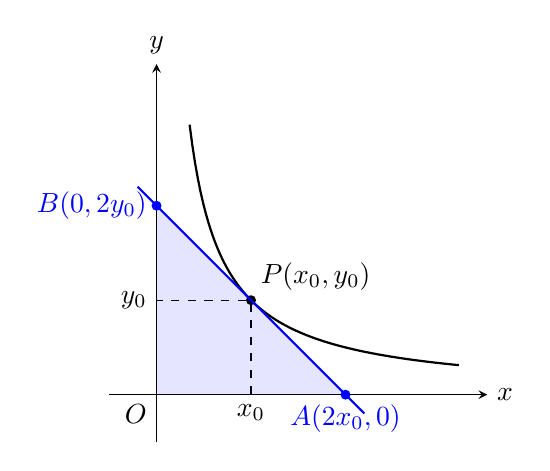
\begin{tikzpicture}[scale=1.2, >=stealth]
            \draw[->] (-0.5,0) -- (3.5,0) node[right] {$x$};
            \draw[->] (0,-0.5) -- (0,3.5) node[above] {$y$};
            \node[below left] at (0,0) {$O$};
            \draw[thick, domain=0.35:3.2, samples=100] plot (\x, {1/\x});
            \node[above right] at (1,1) {$P(x_0, y_0)$};
            \fill (1,1) circle (1.5pt);
            \draw[dashed] (1,0) node[below] {$x_0$} -- (1,1) -- (0,1) node[left] {$y_0$};
            \draw[thick, blue] (-0.2, 2.2) -- (2.2, -0.2);
            \fill[blue] (2,0) circle (1.5pt) node[below] {$A(2x_0, 0)$};
            \fill[blue] (0,2) circle (1.5pt) node[left] {$B(0, 2y_0)$};
            \fill[opacity=0.1, blue] (0,0) -- (2,0) -- (0,2) -- cycle;
        \end{tikzpicture}
    \end{center}

    对 $y = \frac{1}{x}$ 求导得 $y' = -\frac{1}{x^2}$，故点 $P$ 处的切线斜率为
    \begin{equation}
        k = -\frac{1}{x_0^2}.
    \end{equation}
    切线方程为
    \begin{equation}
        y - y_0 = -\frac{1}{x_0^2}(x - x_0) \implies \frac{x}{x_0^2} + y = \frac{2}{x_0}.
    \end{equation}
    两端同除以 $\frac{2}{x_0}$，整理为截距式：
    \begin{equation}
        \frac{x}{2x_0} + \frac{y}{2y_0} = 1.
    \end{equation}
    切线与两坐标轴的交点分别为 $A(2x_0, 0)$ 与 $B(0, 2y_0)$．

    切线与两坐标轴所围成三角形的面积为
    \begin{equation}
        S = \frac{1}{2} |OA| \cdot |OB| = \frac{1}{2} |2x_0| \cdot |2y_0| = 2|x_0 y_0| = 2 \cdot 1 = 2.
    \end{equation}
    故面积恒为定值 $2$．
\end{myproof}

\begin{problem}{正圆锥容器注水上升速率}{Cone-Water-Level-Rising-Rate}
    有一底半径为 $r\text{ cm}$，高为 $h\text{ cm}$ 的正圆锥形容器，现以 $a\text{ cm}^3/\text{s}$ 的速度自顶部向其内注水，求水面上升的速度．
\end{problem}

\begin{solution}
    设某时刻水深为 $x\text{ cm}$（$0 < x < h$），水面上升速度为 $\frac{\d x}{\d t}$．

    由相似三角形性质，此时水面的截面圆半径为
    \begin{equation}
        \rho = \frac{r}{h} x.
    \end{equation}
    容器内水的体积为
    \begin{equation}
        V = \frac{1}{3}\uppi \rho^2 x = \frac{\uppi r^2}{3h^2} x^3.
    \end{equation}
    两端对时间 $t$ 求导，得
    \begin{equation}
        \frac{\d V}{\d t} = \frac{\uppi r^2}{h^2} x^2 \frac{\d x}{\d t}.
    \end{equation}
    已知注水速度 $\frac{\d V}{\d t} = a\text{ cm}^3/\text{s}$，代入解得
    \begin{equation}
        \frac{\d x}{\d t} = \frac{a h^2}{\uppi r^2 x^2}.
    \end{equation}
    \begin{equation}
        \boxed{\frac{\d x}{\d t} = \frac{a h^2}{\uppi r^2 x^2}\text{ cm}/\text{s}.}
    \end{equation}
\end{solution}

\begin{problem}{漏斗与圆柱形筒的相关变化率}{Related-Rates-Funnel-And-Cylinder}
    水自高为 $18\text{ cm}$，底半径为 $6\text{ cm}$ 的圆锥形漏斗流入直径为 $10\text{ cm}$ 的圆柱形筒中．已知水在漏斗中深度为 $12\text{ cm}$ 时水平面下降的速率为 $1\text{ cm}/\text{m}$．试求圆柱形筒中水平面上升的速度．
\end{problem}

\begin{solution}
    设 $t$ 时刻漏斗中水深为 $H$，漏斗中水的体积为 $V_1$；圆柱形筒中水深为 $h$，圆柱形筒中水的体积为 $V_2$．

    漏斗内水面半径为 $R = \frac{6}{18}H = \frac{1}{3}H$，故漏斗中水的体积为
    \begin{equation}
        V_1 = \frac{1}{3}\uppi R^2 H = \frac{\uppi}{27} H^3.
    \end{equation}
    两端对时间 $t$ 求导：
    \begin{equation}
        \frac{\d V_1}{\d t} = \frac{\uppi}{9} H^2 \frac{\d H}{\d t}.
    \end{equation}
    当 $H = 12\text{ cm}$ 且 $\frac{\d H}{\d t} = -1\text{ cm}/\text{m}$ 时，漏斗出水速率为
    \begin{equation}
        -\frac{\d V_1}{\d t} = -\frac{\uppi}{9} (12)^2 (-1) = 16\uppi\text{ cm}^3/\text{m}.
    \end{equation}
    圆柱形筒的底面半径为 $r = 5\text{ cm}$，筒内水的体积为
    \begin{equation}
        V_2 = \uppi r^2 h = 25\uppi h.
    \end{equation}
    两端对时间 $t$ 求导：
    \begin{equation}
        \frac{\d V_2}{\d t} = 25\uppi \frac{\d h}{\d t}.
    \end{equation}
    由水量守恒，$\frac{\d V_2}{\d t} = -\frac{\d V_1}{\d t}$，得
    \begin{equation}
        25\uppi \frac{\d h}{\d t} = 16\uppi \implies \frac{\d h}{\d t} = \frac{16}{25} = 0.64\text{ cm}/\text{m}.
    \end{equation}
    \begin{equation}
        \boxed{\frac{\d h}{\d t} = \frac{16}{25}\text{ cm}/\text{m} \quad (\text{即 } 0.64\text{ cm}/\text{m}).}
    \end{equation}
\end{solution}

\endinput
